%--- Implementation
\begin{figure}[h!]
    \centering
    \caption{Geographic Spillovers of \emph{Plan Cuadrante} on Neighboring Untreated Municipalities}
    \label{fig:spillover_admin}
    \begin{subfigure}{0.495\textwidth}
        \centering
        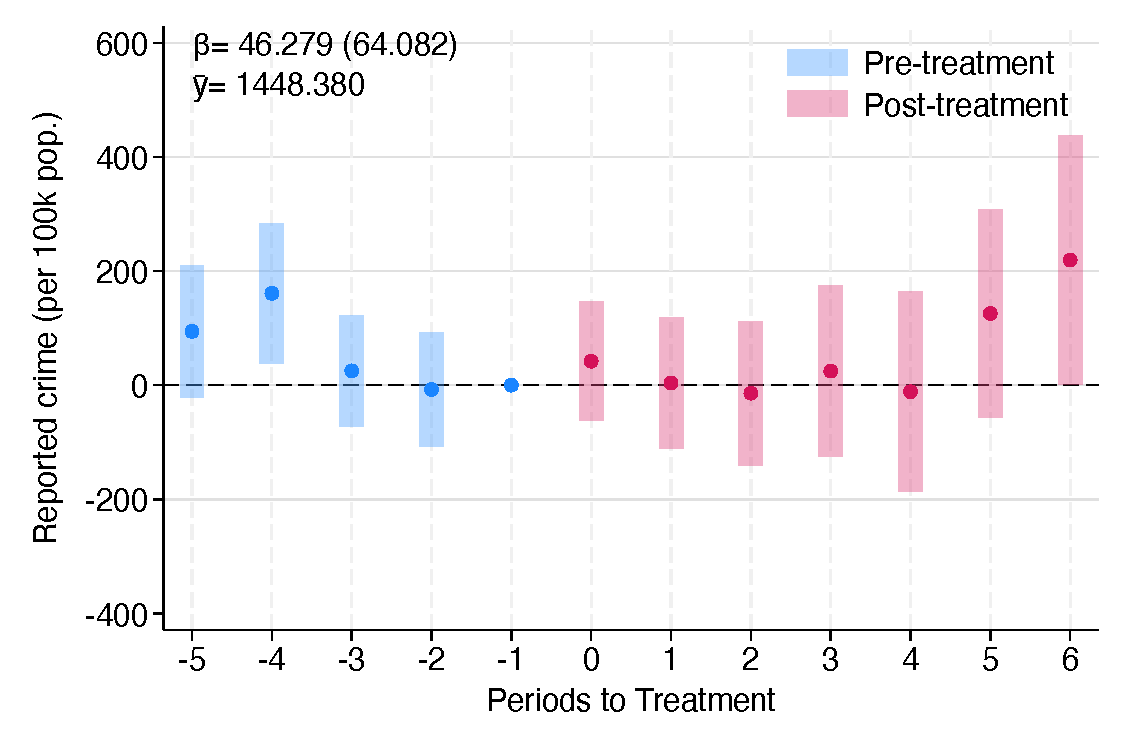
\includegraphics[width=0.98\textwidth]{../manuscript/Graphs/totalreportedcrime_allcomunas_neighbors.pdf}
        \caption{Spillovers on Reported crime}
    \end{subfigure}%
    ~ 
    \begin{subfigure}{0.495\textwidth}
    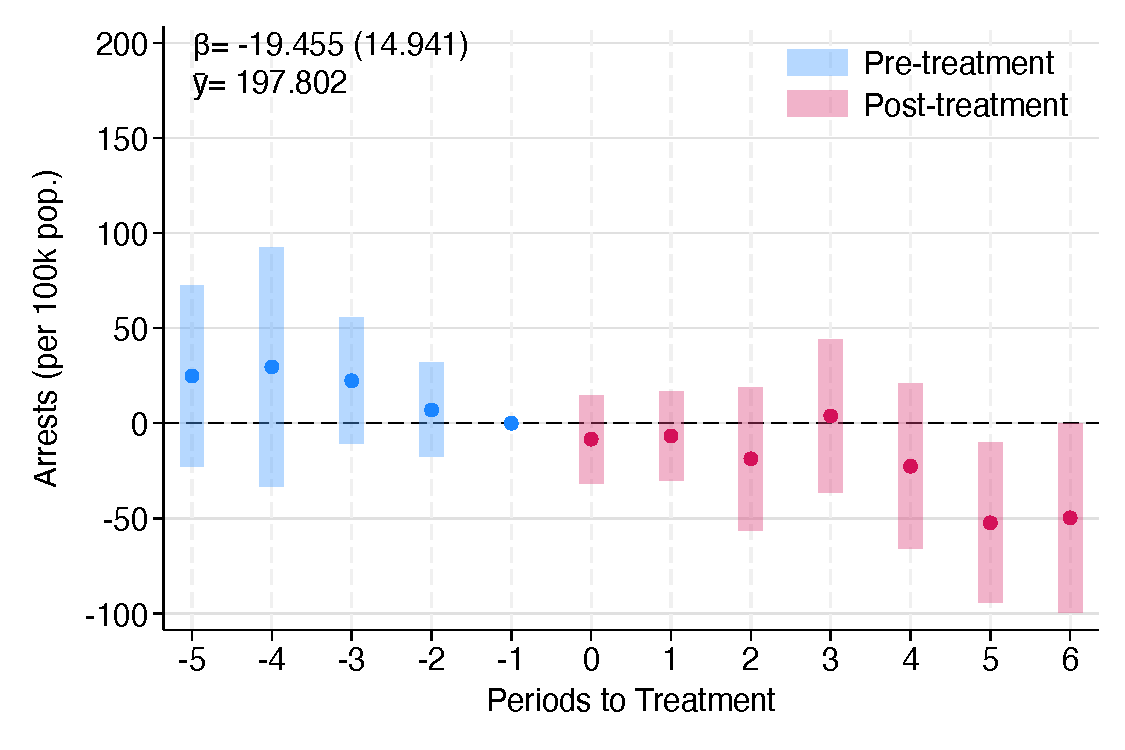
\includegraphics[width=0.98\textwidth]{../manuscript/Graphs/totalarrestscrime_allcomunas_neighbors.pdf}
        \caption{Spillovers on Arrests}
    \end{subfigure}
    \begin{subfigure}{0.495\textwidth}
        \centering
        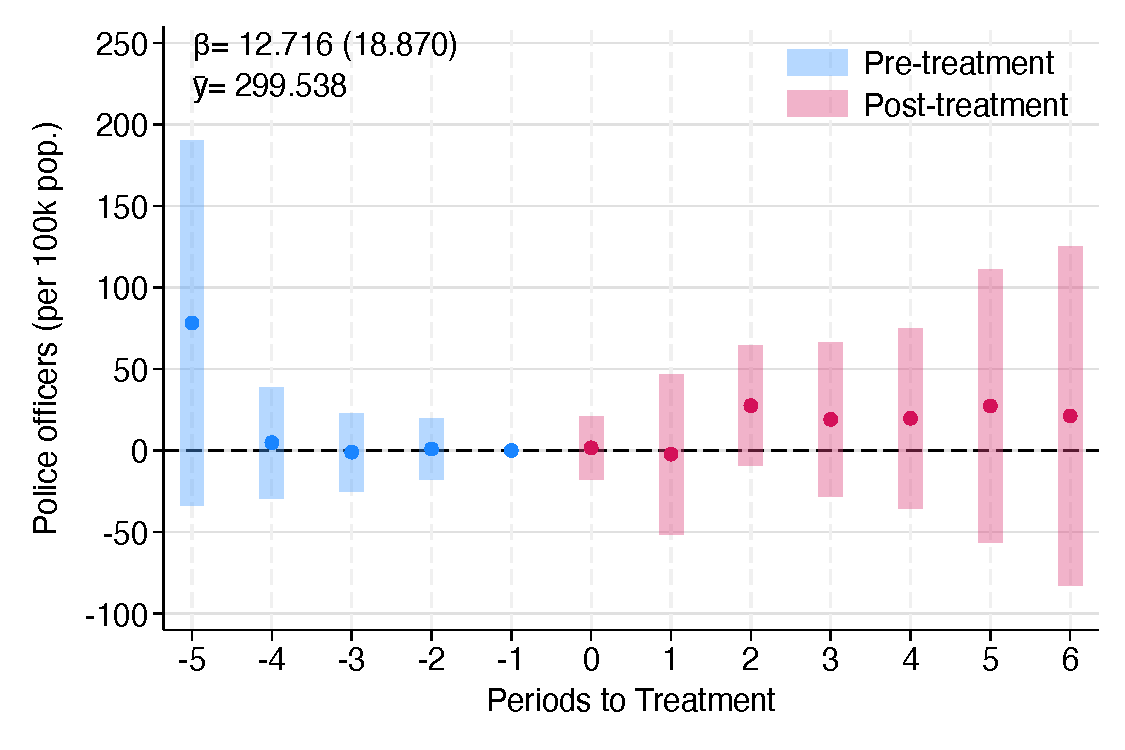
\includegraphics[width=0.98\textwidth]{../manuscript/Graphs/dotpc_allcomunas_neighbors.pdf}
        \caption{Spillovers on Police Officers}
    \end{subfigure}%
    ~ 
    \begin{subfigure}{0.495\textwidth}
    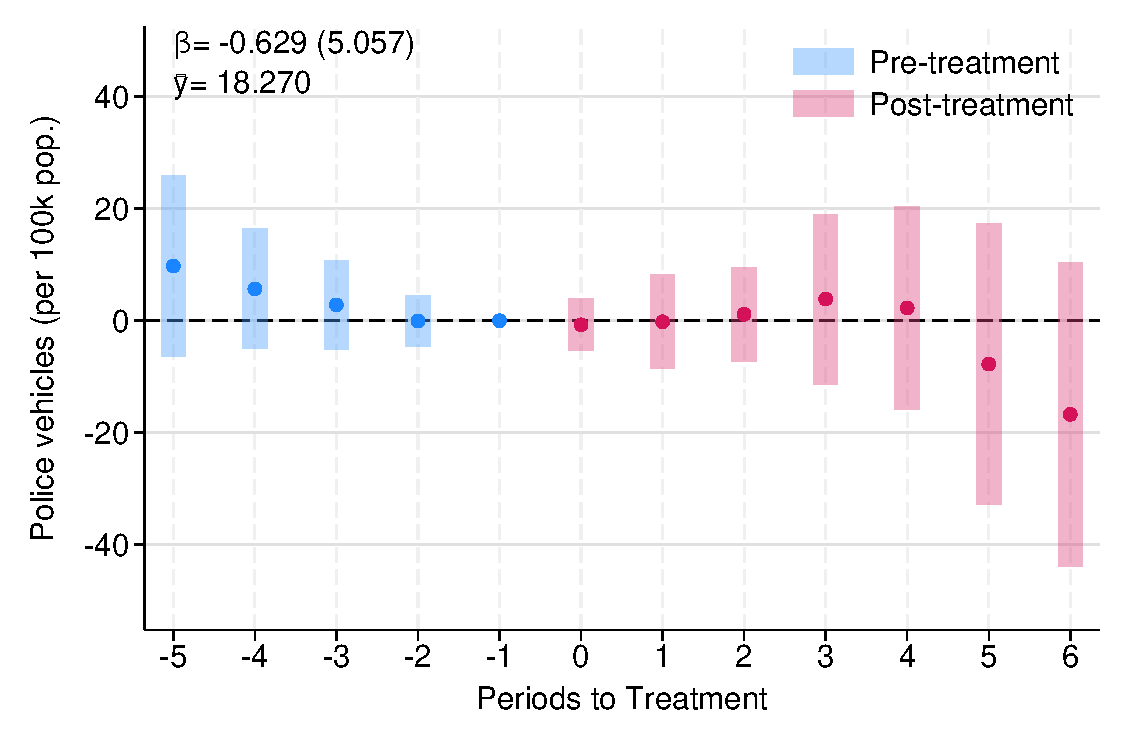
\includegraphics[width=0.98\textwidth]{../manuscript/Graphs/vehiclespc_allcomunas_neighbors.pdf}
        \caption{Spillovers on Patrol Vehicles}
    \end{subfigure}
    \begin{minipage}{0.9\textwidth}
    \footnotesize
    Notes: This figure reports the spillover effects of \emph{Plan Cuadrante} on the number of crimes reported to the police in the municipality per 100,000 inhabitants (panel a), the number of arrests in the municipality per 100,000 inhabitants (panel b), the number of police officers per 100,000 inhabitants (panel c), and the number of patrol vehicles per 100,000 inhabitants (panel d). Panels (a)--(d) include 2,859, 2,166, 1,144, and 1,942 observations respectively. Specifically, the figure shows the dynamic effects of the \emph{Plan Cuadrante} for neighbor municipalities which never introduced the program. The estimation is conducted using the procedure developed in \citet{Callaway} for difference-in-differences with staggered treatment adoption, using as the treatment introduction date the earliest date of a neighboring municipality. The dots in the figure represent the estimated coefficients and the bars behind them 95\% confidence intervals. Standard errors are clustered at the municipality level using the wild bootstrapping procedure. The pooled effect and the mean outcome before the introduction of the treatment for every outcome is also presented in each panel. 
    \end{minipage}
\end{figure}
